++\documentclass[12pt]{article}
\setlength\parindent{0pt}
\usepackage{fullpage}
%\usepackage[margin=0.5in, paperwidth=13.5in, paperheight=8.4375in]{geometry}
\usepackage[margin=0.5in, paperwidth=8.5in, paperheight=11in]{geometry}

\usepackage{amsmath}
\usepackage{graphicx}
\newcommand{\BI}{\begin{itemize}}
\newcommand{\insp}{\vspace{1in}}
\newcommand{\EI}{\end{itemize}}
\newcommand{\BE}{\begin{enumerate}}
\newcommand{\EE}{\end{enumerate}}
\newcommand{\BS}{\bigskip}
\setlength{\parskip}{4mm}


\pagenumbering{gobble}

\begin{document}

\begin{center}
	\Large \sc Homework Quiz 1 - Stellar Motion (form B)
\end{center}

\begin{flushright}
	Name: \underline{\hspace{4in}}
\end{flushright}

\it Instructions: Answer the question on the front and the two questions on the back. 

\rm
	
	\begin{enumerate}
		\item Today in Syracuse (latitude $43^\circ$ N) the Sun will rise very close to due east. {\it (Note that these diagrams have the east/west typo corrected, so you don't need to do that.)} 
		
		\begin{center}
		\begin{minipage}{0.45\textwidth}
			\begin{center}
\it Sky Above Horizon\\
				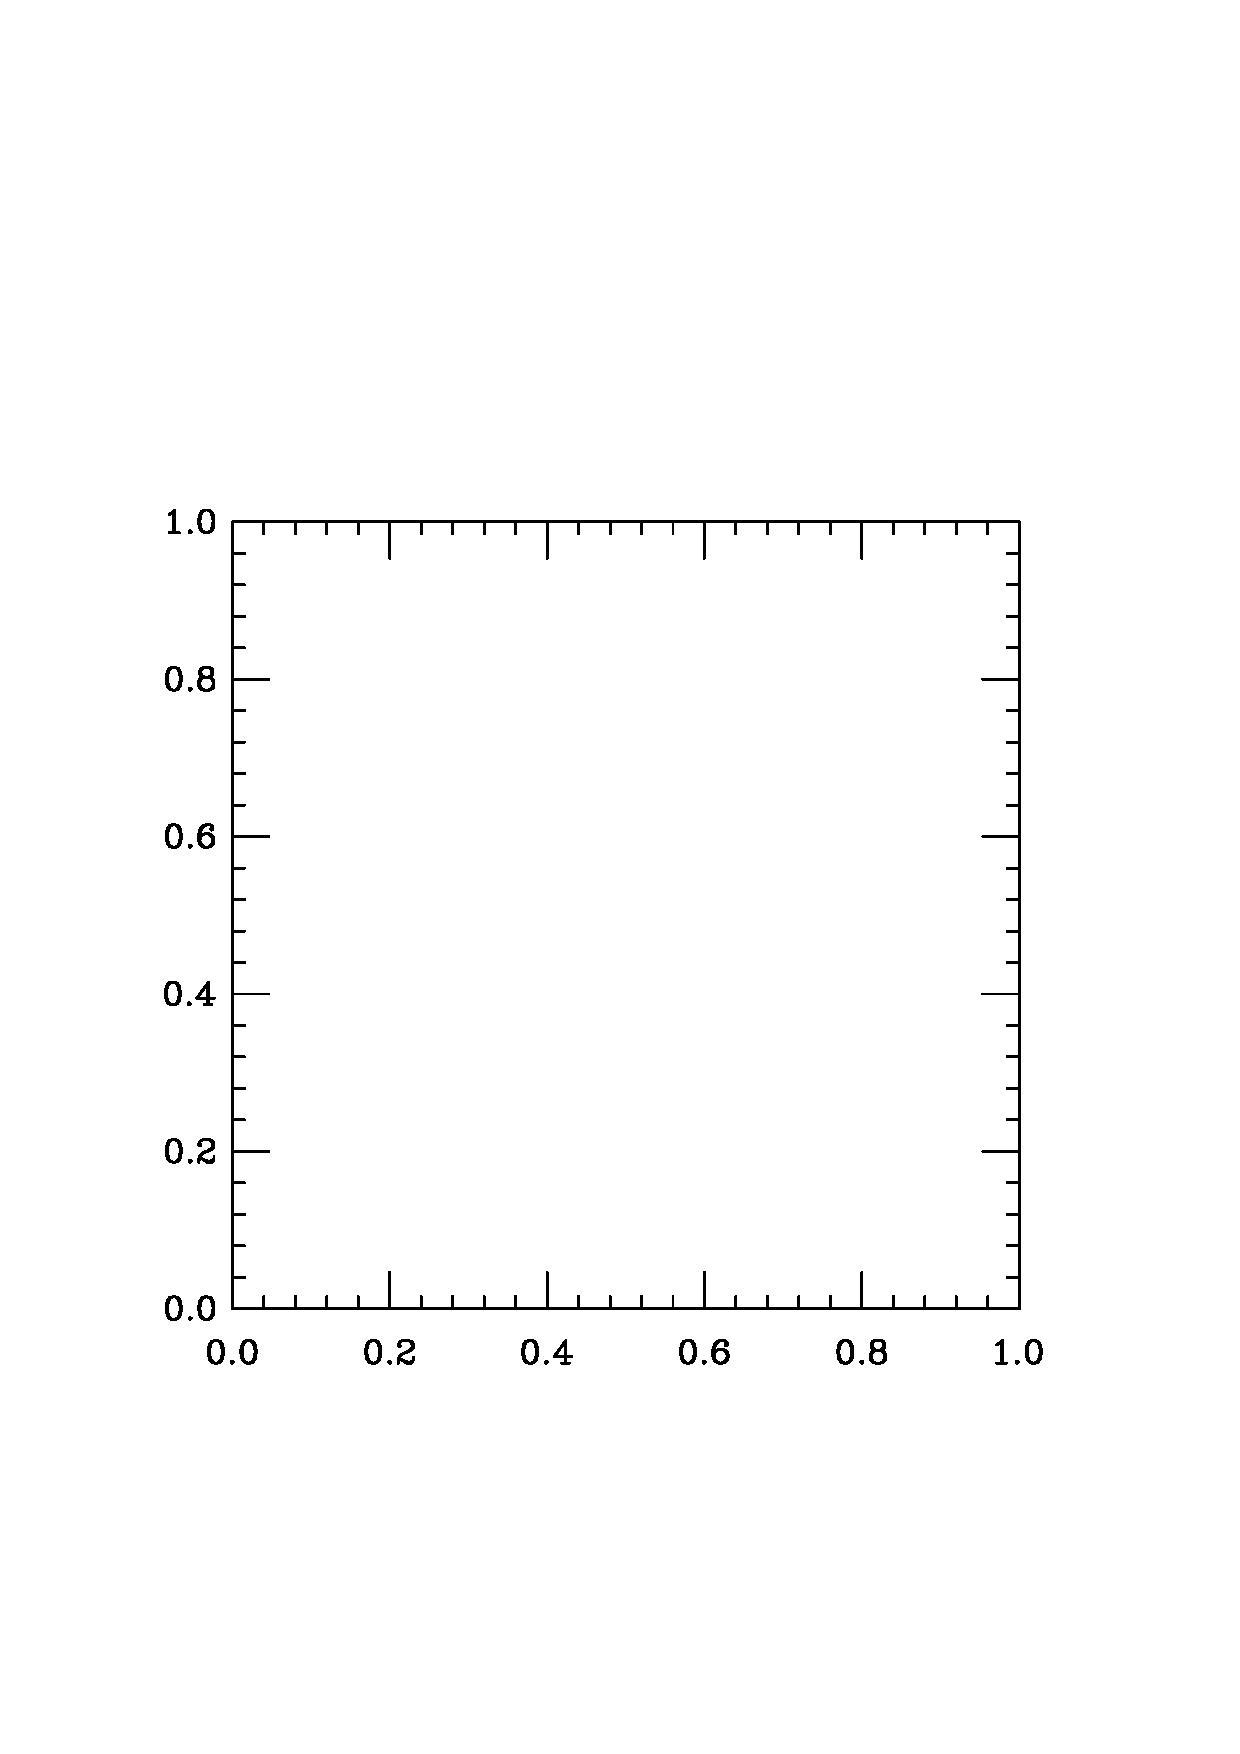
\includegraphics[width=0.9\textwidth]{topsky-crop.pdf}
			\end{center}
		\end{minipage}
		\begin{minipage}{0.45\textwidth}
			\begin{center}
				\it Sky Below Horizon\\
				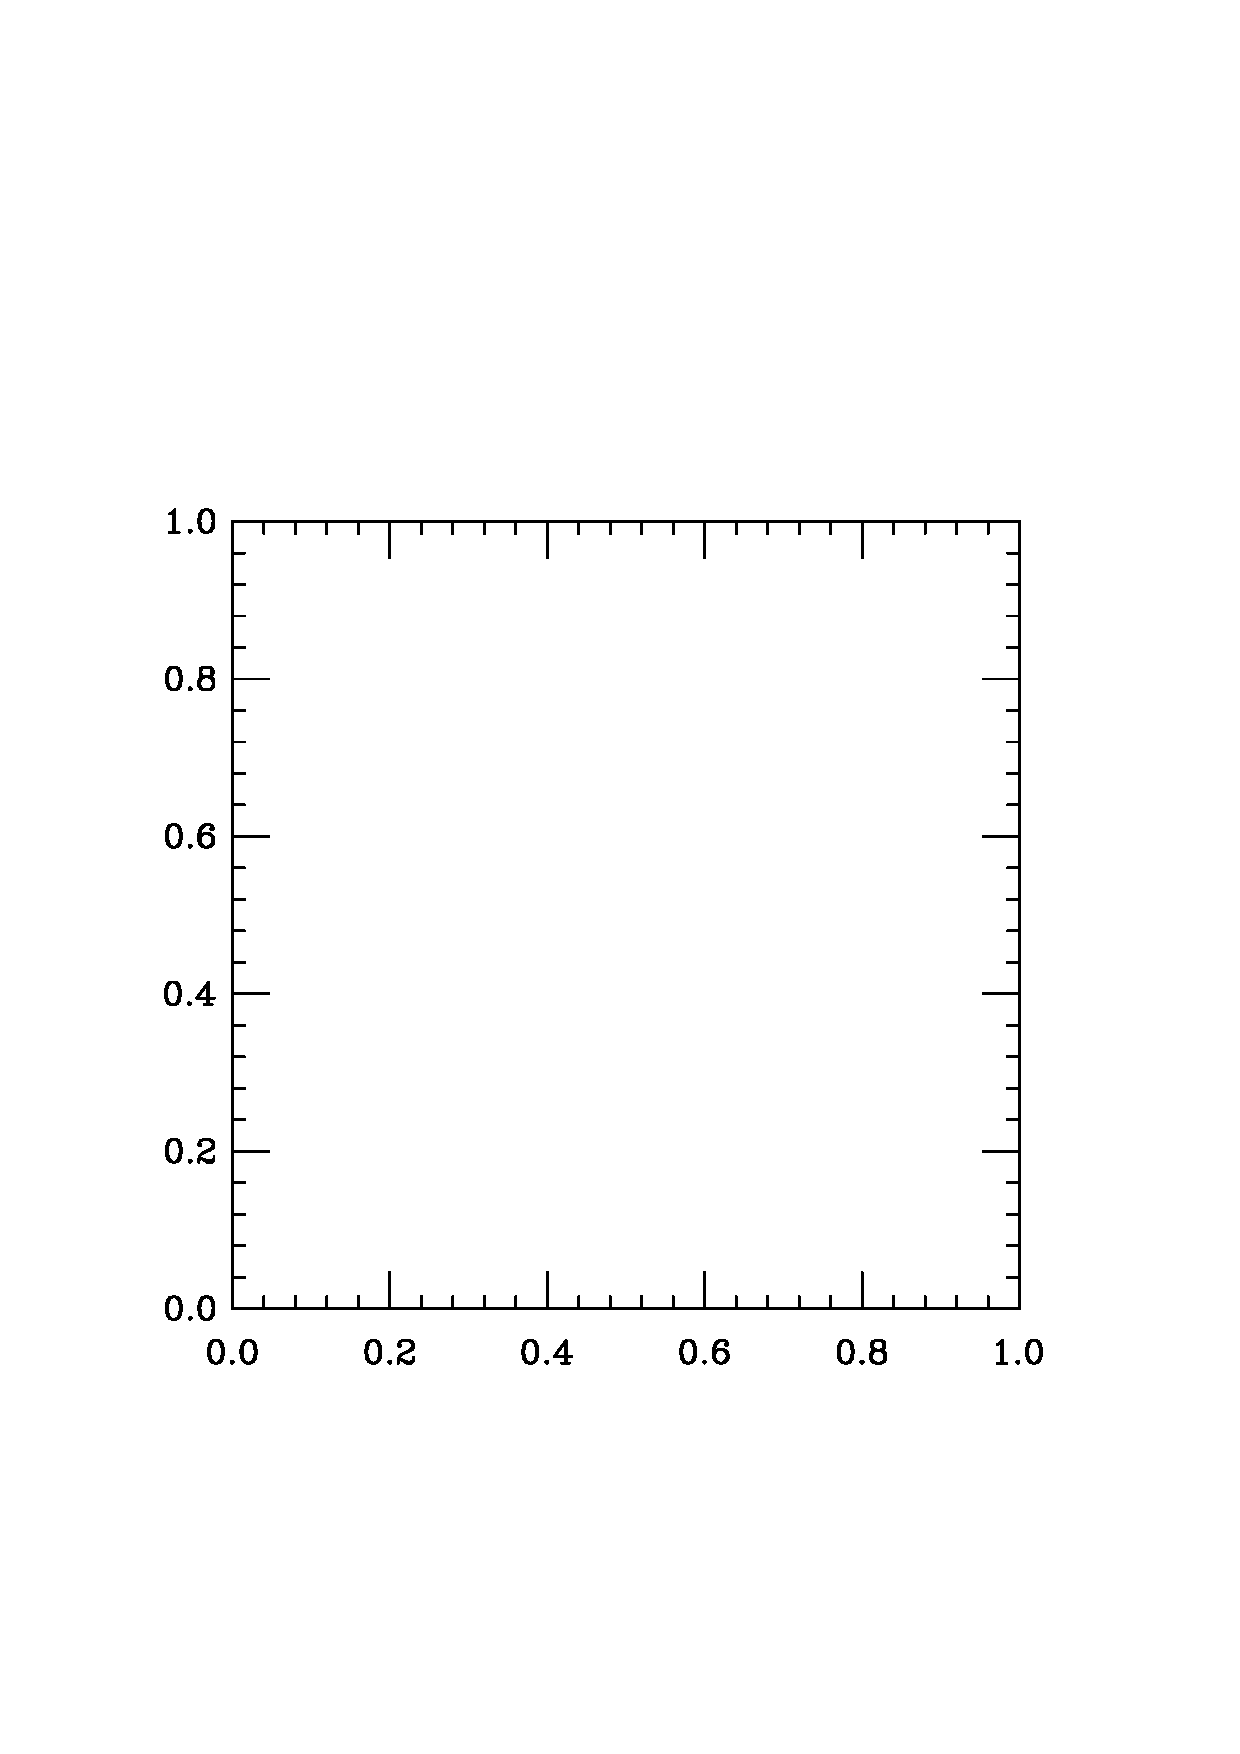
\includegraphics[width=0.9\textwidth]{botsky-crop.pdf}
			\end{center}
		\end{minipage}
		\end{center}
		
		Draw the path of the Sun over 24 hours. Then label where it will be at midnight, and describe in words where it is. 
		
		\newpage
		
		\item Where would an observer at the South Pole find the North Celestial Pole? Where would they find the South Celestial Pole? {\it (You may describe clearly in words and/or label on the diagrams.)}
		
				\begin{center}
			\begin{minipage}{0.4\textwidth}
				\begin{center}
					\it Sky Above Horizon\\
					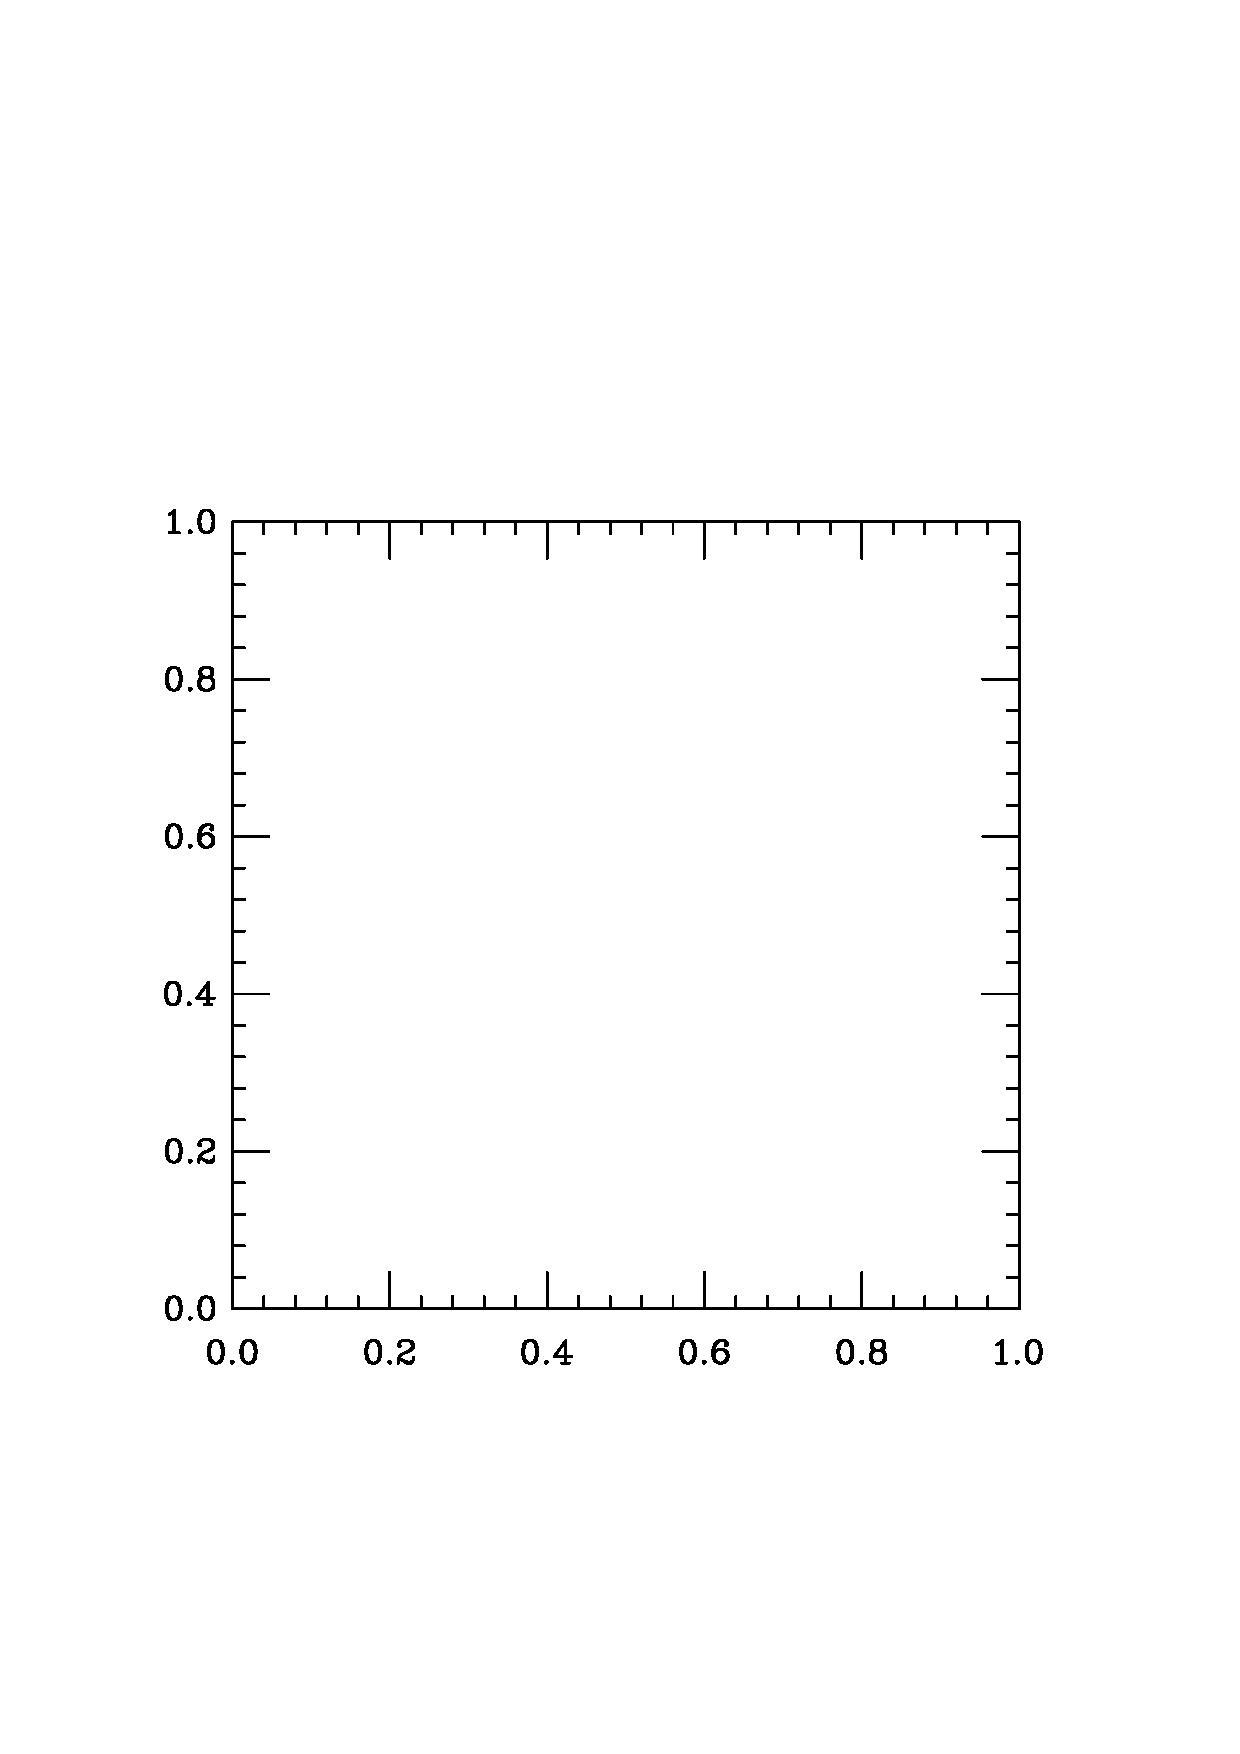
\includegraphics[width=0.8\textwidth]{topsky-crop.pdf}
				\end{center}
			\end{minipage}
			\begin{minipage}{0.4\textwidth}
				\begin{center}
					\it Sky Below Horizon\\
					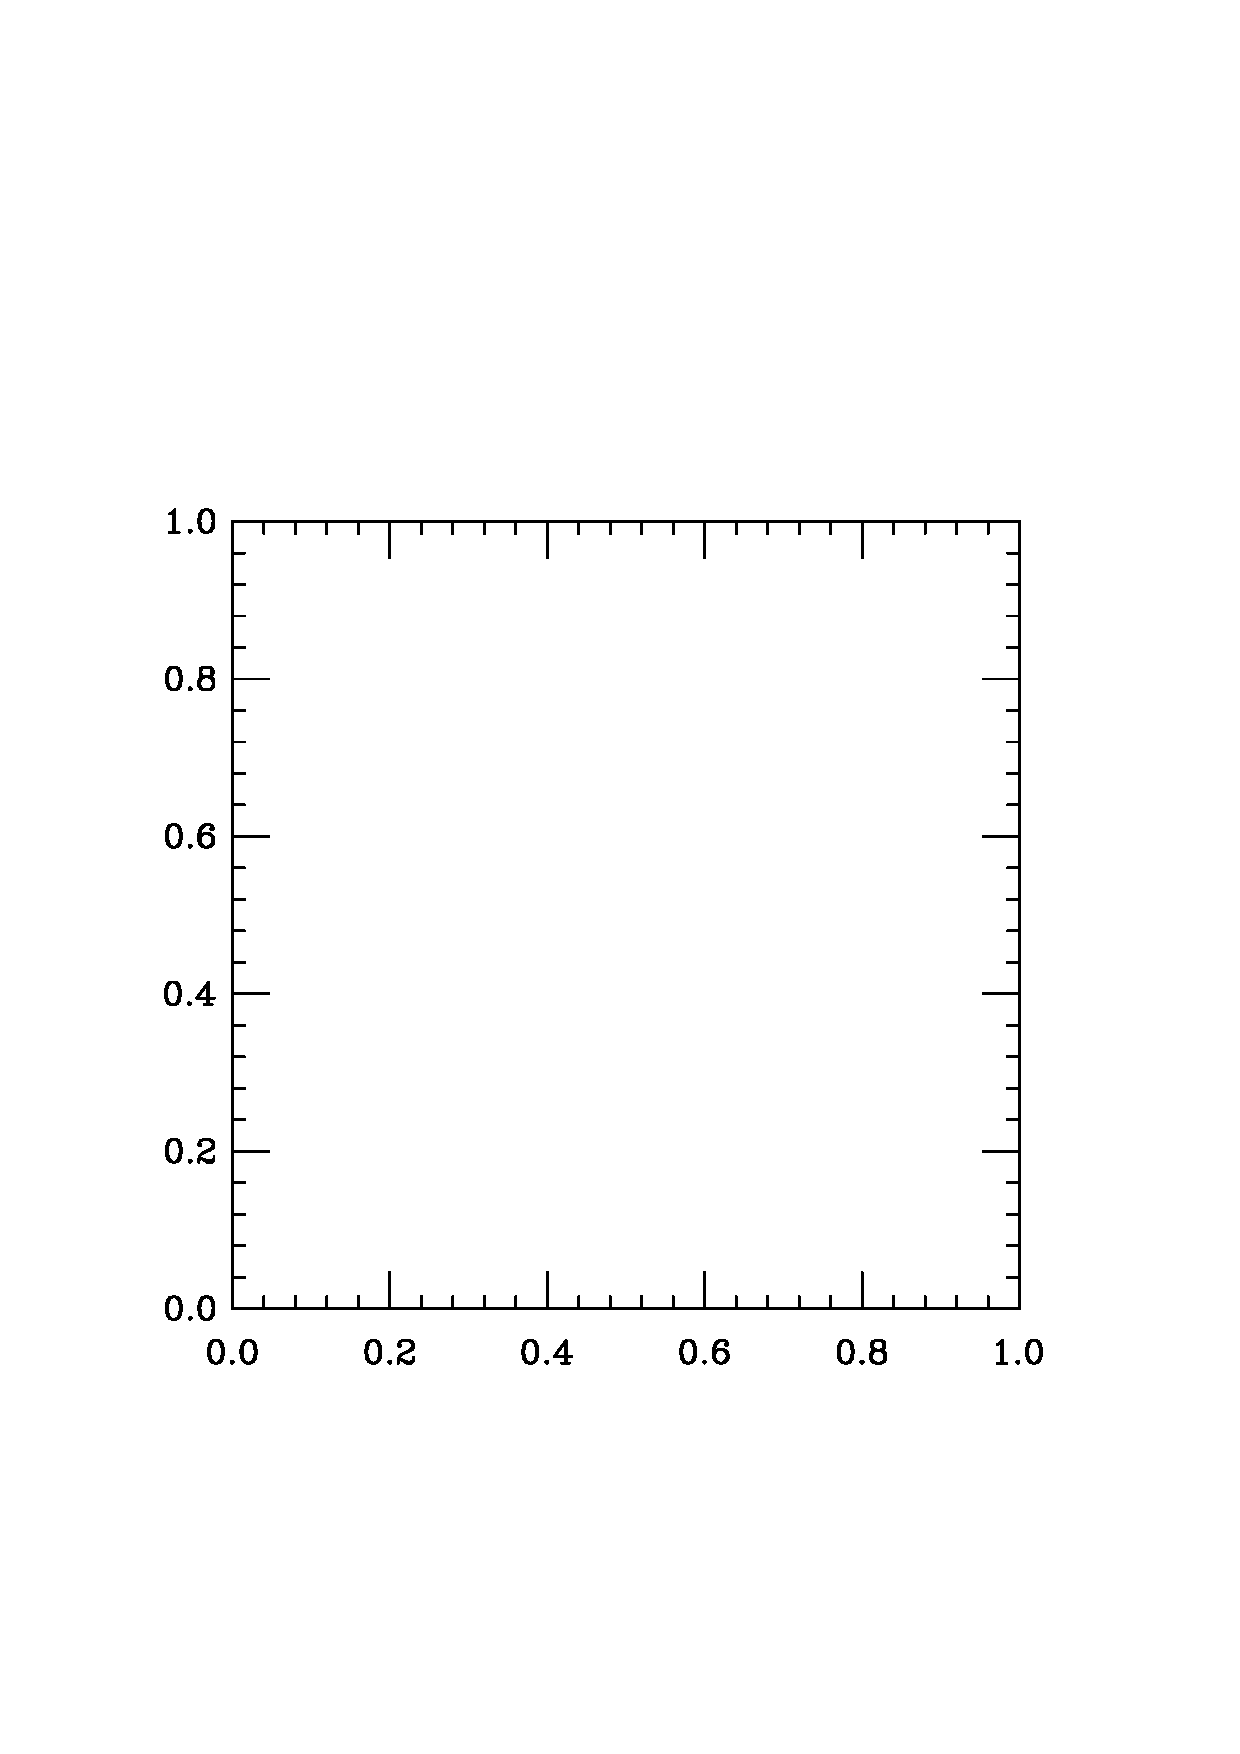
\includegraphics[width=0.8\textwidth]{botsky-crop.pdf}
				\end{center}
			\end{minipage}
		\end{center}
		
		
		\vspace{1.5in}
		
		\item As seen from Syracuse (latitude $43^\circ N$), the star Navi is always above the horizon; it moves in a counterclockwise circle around the North Celestial Pole, but never rises or sets.
		
		How would someone in Quito, Ecuador (very near the Equator) see Navi move? Draw its path on the diagrams below. 
		
						\begin{center}
			\begin{minipage}{0.4\textwidth}
				\begin{center}
					\it Sky Above Horizon\\
					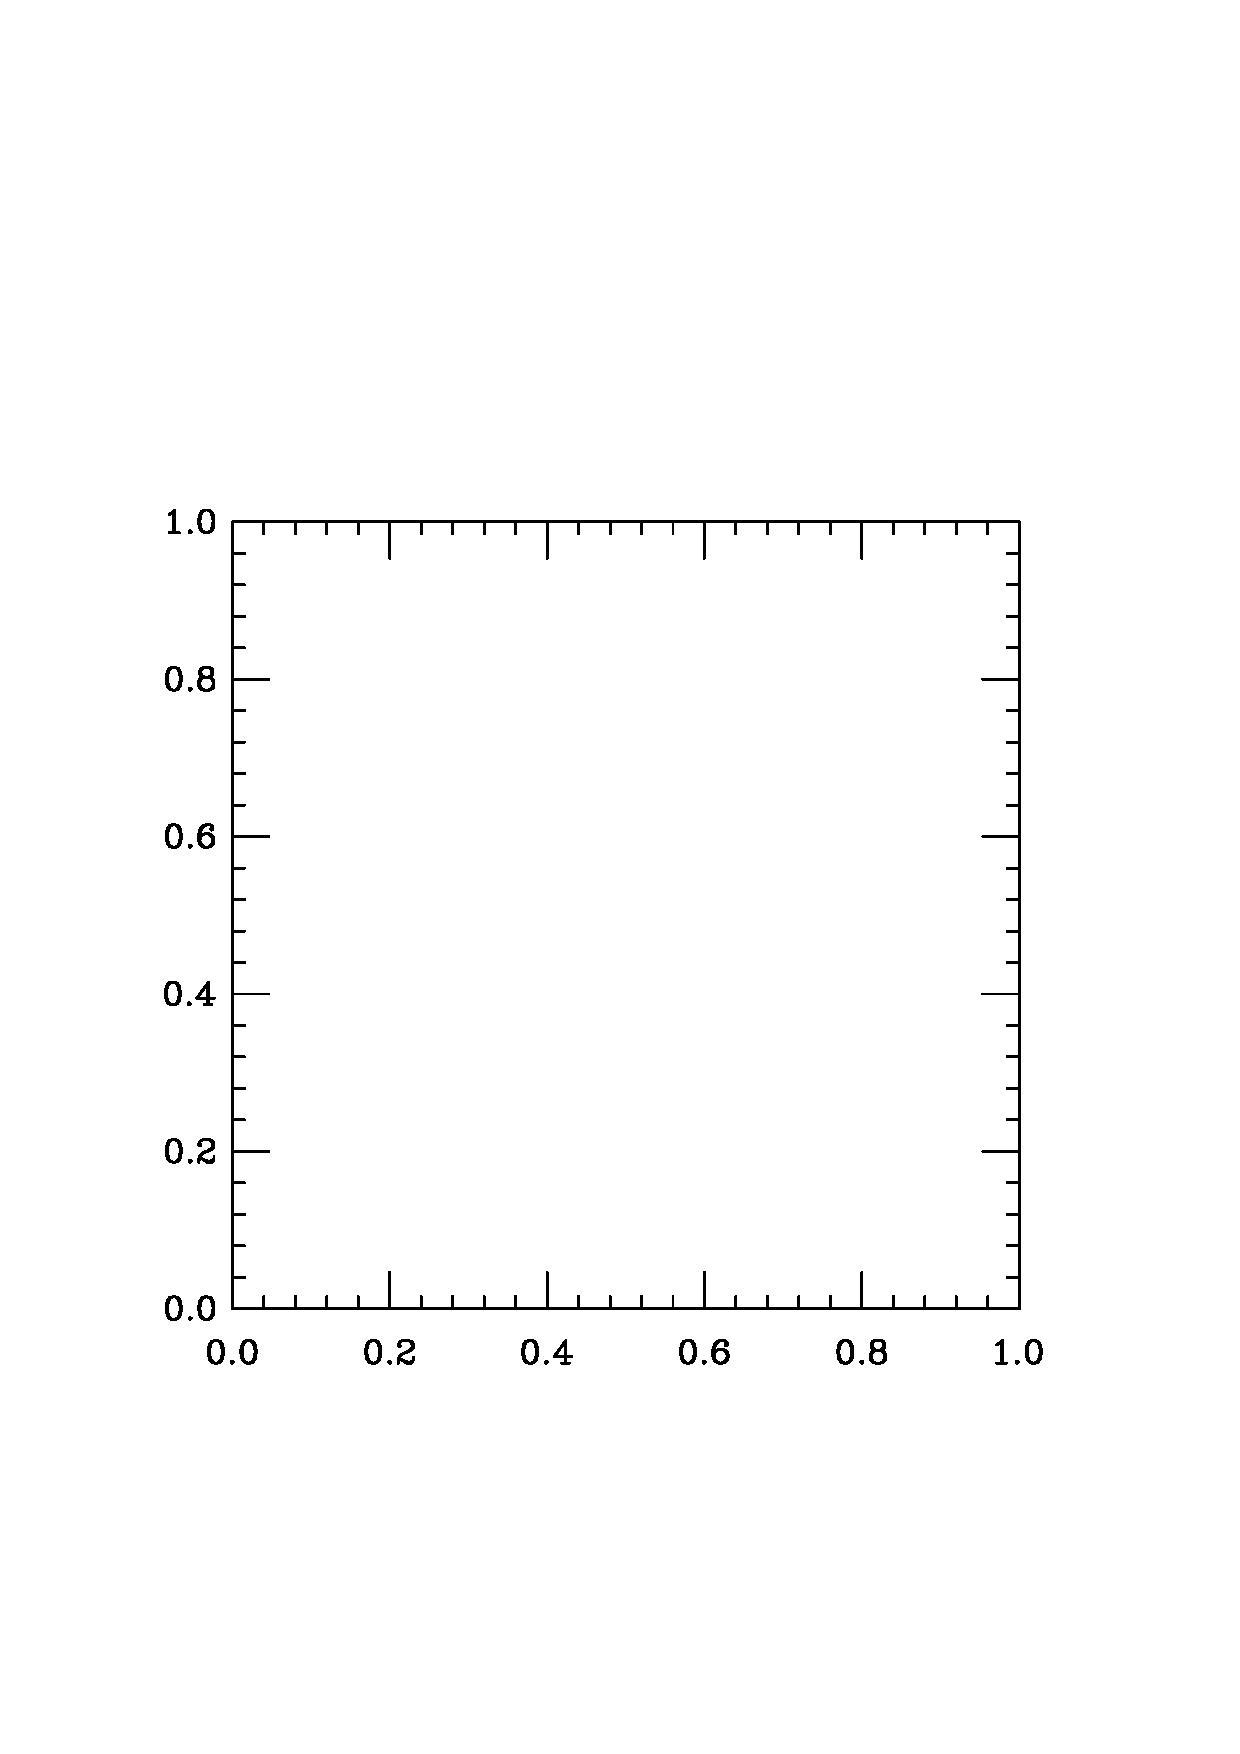
\includegraphics[width=0.8\textwidth]{topsky-crop.pdf}
				\end{center}
			\end{minipage}
			\begin{minipage}{0.4\textwidth}
				\begin{center}
					\it Sky Below Horizon\\
					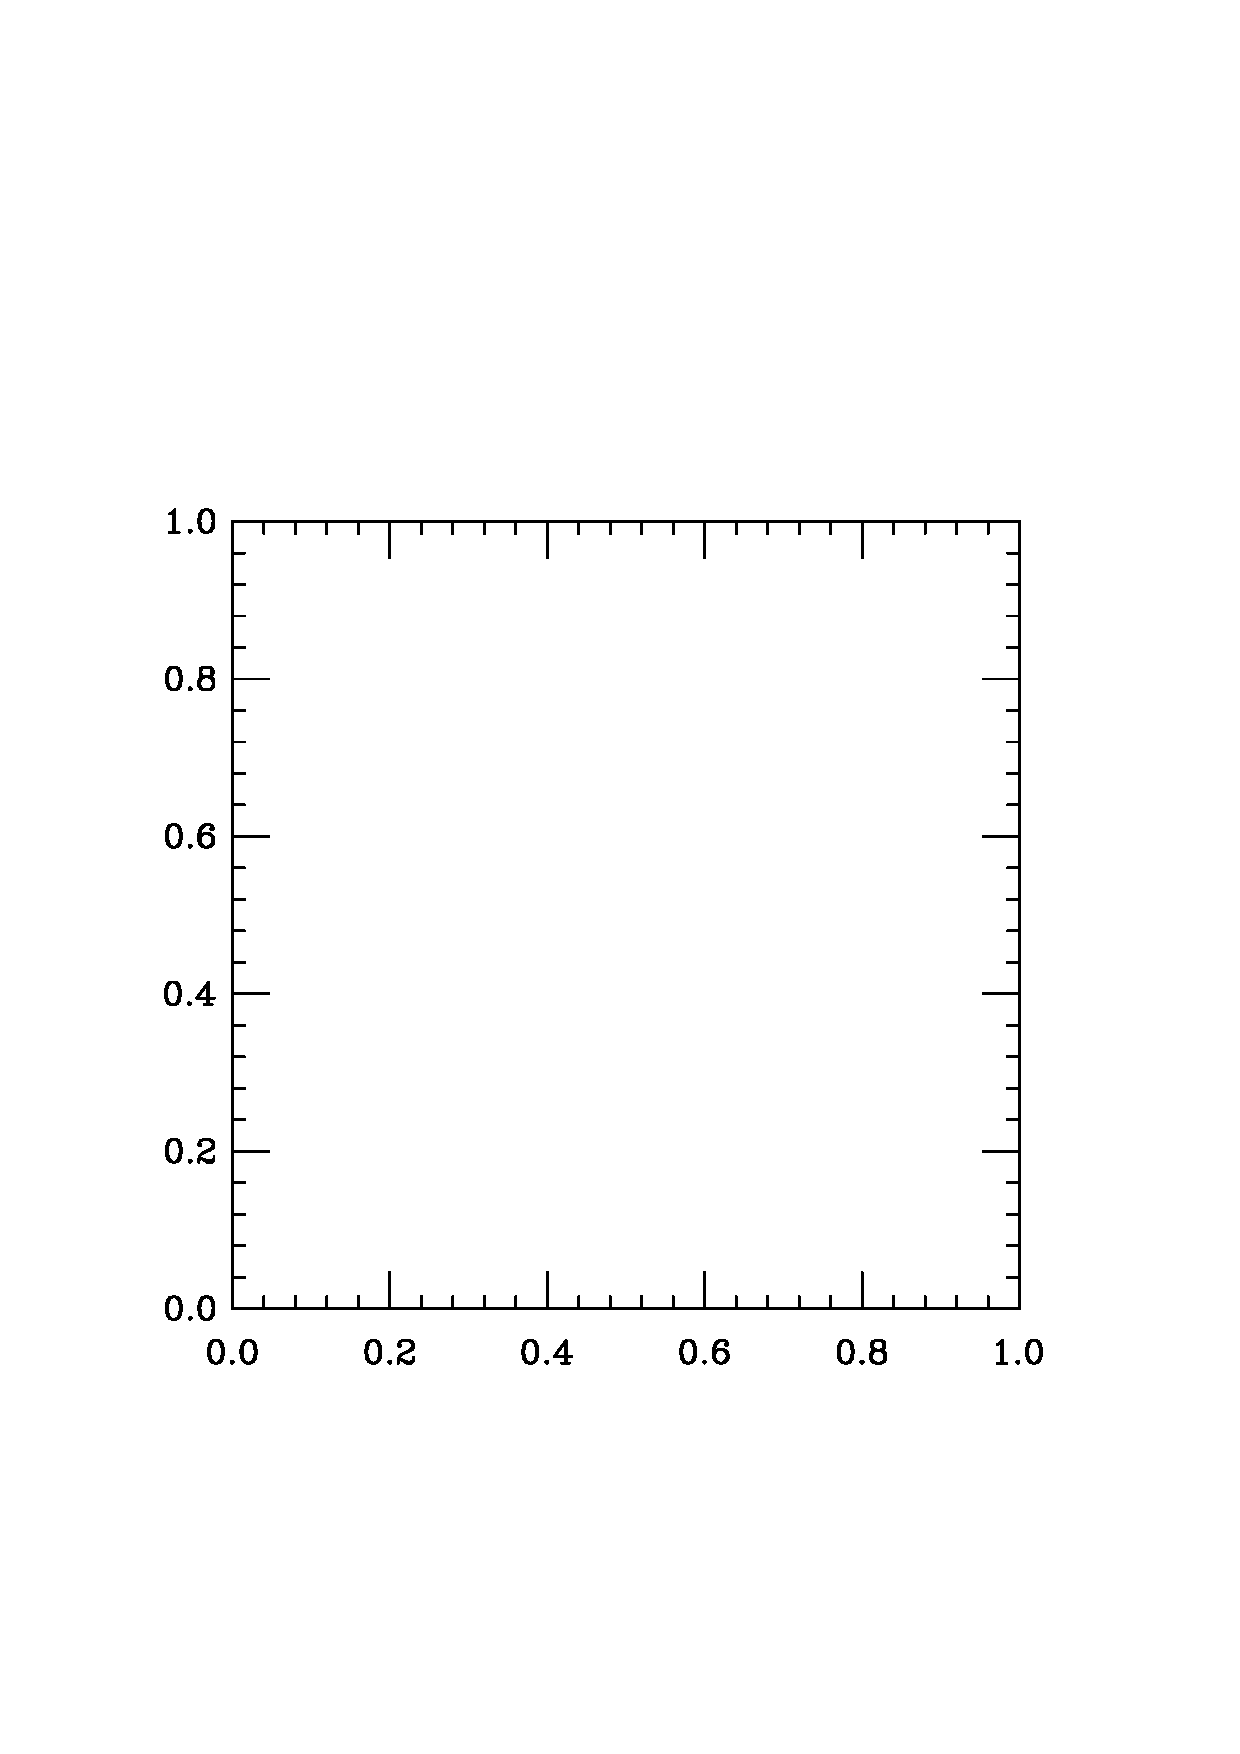
\includegraphics[width=0.8\textwidth]{botsky-crop.pdf}
				\end{center}
			\end{minipage}
		\end{center}
		
	\end{enumerate}
	
	
		
		
		
	
\end{document}
	
	
	
	